\workshopexclude{\section{Large Language Models are Human-Level Prompt Engineers}}
\workshoponly{\section{Additional Experimental Results}\label{app:add_res} }
This section examines how APE can guide LLMs to desired behaviors. We investigate from four perspectives: zero-shot performance, few-shot in-context learning performance, zero-shot chain-of-thought reasoning, and truthfulness. Our experiments show that APE can find prompts that improve task performance, performing equal to or even better than those authored by humans. APE also often produces insightful tricks for how to best prompt language models that can be successfully transferred to new tasks (see Section \ref{sec:cot}).
\workshoponly{For consistency, we duplicate some of the results here.}

\subsection{Instruction Induction}\label{sec:inst_induct}
We assess the effectiveness of zero-shot and few-shot in-context learning on 24 instruction induction tasks proposed in \citet{honovich2022instruction}. The tasks span many facets of language understanding, from simple phrase structure to similarity and causality identification. We provide a detailed descriptions of each task in Appendix B. For each task, we sample five input-output pairs from the training data and select the best instruction using algorithm \ref{alg:ape}. Then, we evaluate the quality of the instruction by executing the instruction on InstructGPT \footnote{We use the \textit{text-davinci-002} via the OpenAI API (\url{https://beta.openai.com/}). Though not stated explicitly in the API, we assume the models are those reported by \citet{ouyang2022training}.}. We repeat our experiments five times with different random seeds to report the mean and standard deviation. The exact templates for our experiments can be found in Appendix (Table \ref{table:raw_templates}).

\begin{figure}[t]
  \vspace{-0.25in}
  \centering
  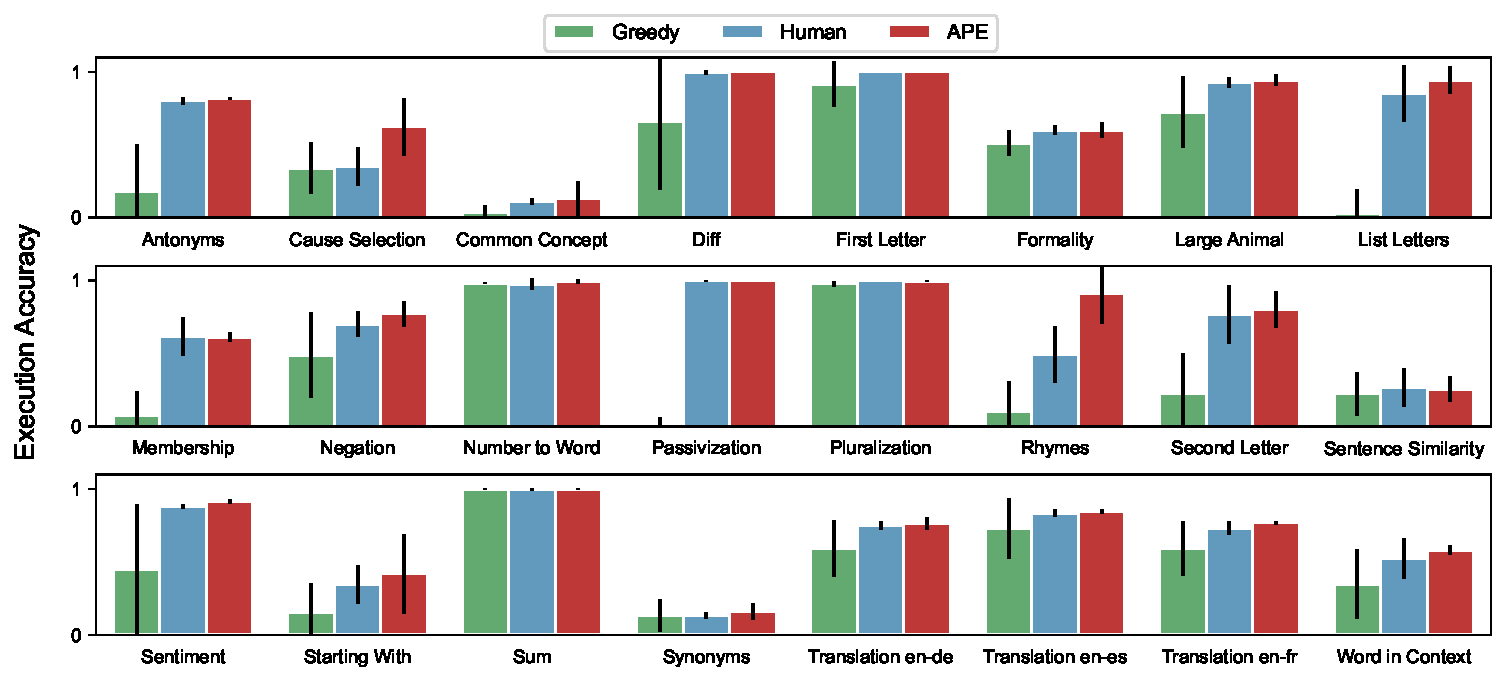
\includegraphics[width=0.95\linewidth]{figures/main/exec_acc_zero_shot.pdf}
  \caption{Zero-shot test accuracy on 24 Instruction Induction tasks. \algname~achieves human-level or better performance on all  24 out of 24 tasks.}\label{fig:main-zero-shot}
\end{figure}

\paragraph{Zero-shot Learning}
We compare our method against two baselines: human prompt engineers (Human)\footnote{\mbox{We use the gold annotations from \citet{honovich2022instruction}, which were manually verified for correctness.}} and the model-generated instruction algorithm proposed by \citet{honovich2022instruction}. This algorithm can be thought of as a greedy version of \algname, without a search and selection process; thus, we refer to it as ``Greedy''. Figure \ref{fig:main-zero-shot} shows the zero-shot performance of InstructGPT using human instructions and model generated instructions. Our algorithm outperforms ``Greedy'' on every task and achieves equal or better than human performance on 24 of 24 tasks. Moreover, the Interquartile Mean (IQM) \citep{agarwal2021deep} across all 24 tasks in Figure \ref{fig:highlight} suggests that \algname~with InstructGPT outperforms human-engineered prompts, obtaining an IQM of 0.810 vs humans' 0.749. We summarize the instruction selected by \algname~for each task in Appendix (Table \ref{table:best_instructions_all}).

% \begin{figure}[t]
%   \vspace{-0.10in}
%   \centering
%   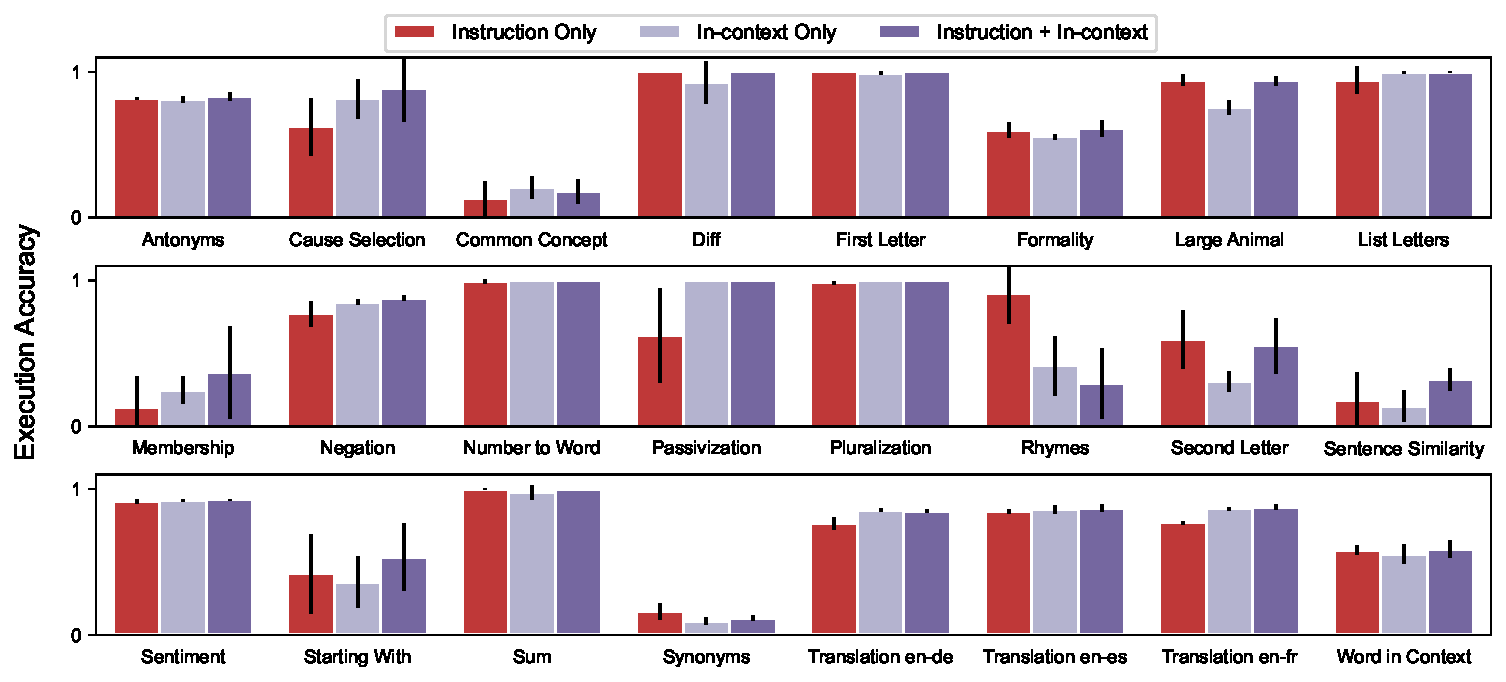
\includegraphics[width=0.95\linewidth]{figures/main/exec_acc_few_shot.pdf}
%   \vspace{-0.10in}
%   \caption{Few-shot in-context test accuracy on 24 Instruction Induction tasks. \algname~improves the few-shot in-context learning performance on 21 out of 24 tasks. See best performing instruction performance in Figure \ref{fig:app-few-shot-best}.}\label{fig:main-few-shot} \vspace{-0.2in}
% \end{figure}

% We observe \algname~can propose varying quality candidates depending on the subset of demonstration chosen for tasks such as Passivization and Start With. 
% % Similar to in-context learning findings \citep{liu2021makes}, a different combination of the in-context examples can yield significantly different results. 
% As shown in Figure \ref{fig:main-zero-shot}, our method achieves worse average performance than humans in Passivization and Sentence Similarity. However, selecting the best instruction still outperforms the human in Figure \ref{fig:app-zero-shot-best}. These results highlight the importance of the initial proposal stage. We found it is crucial to generate instruction candidates based on different demonstrations. Additionally, tasks such as Membership and Second Letter are intrinsically challenging for the model, and \algname~consistently performs worse than humans. 

% \paragraph{Zero-shot Qualitative Analysis}
% To better understand the weaknesses of \algname, we examined instructions in three tasks where \algname~underperforms compared to humans in the zero-shot setting: Passivization, Membership, and Second Letter. As shown in Tables \ref{table:best_instructions}, \ref{table:worst_instructions}, we find large variance in the quality of \algname~instructions due to the difference in demonstration. The best instructions selected by \algname~for each task are semantically correct and recover accuracy relative to humans. In contrast, the worst instructions are all semantically incorrect and perform poorly. Notably, we observe no semantic difference in the demonstrations used to generate the best and worst instruction under inspection.
% This presents further evidence that selecting the right context demonstrations is both vital to some tasks and may escape human intuition, hence the need for an LLM score function.

\paragraph{Few-shot In-context Learning}
We evaluated APE-generated instructions in  few-shot in-context learning, where we insert the instruction before the in-context demonstrations. Those instructions are selected based on zero-shot execution accuracy, and we denote this setting as ``Instruction + In-context'' in Figure \ref{fig:main-few-shot}. As shown in Figure \ref{fig:main-few-shot}, adding an instruction achieves a comparable or better test performance than the standard in-context learning performance on 21 of 24 tasks. Counter-intuitively, adding in-context examples for Rhymes, Large Animal, and Second Letters hurts model performance. We conjecture that it may be because the selected instructions overfit the zero-shot learning scenario and thus do not perform well on the few-shot case. Therefore, we experiment using few-shot execution accuracy as the selection metric. Figure \ref{fig:app-few-shot-as-metric} shows that the few-shot metric achieves comparable or slightly better than the zero-shot metric except for Rhymes. To have an intuitive understanding of what is happening, we provide a qualitative analysis in Appendix \ref{sec:app_ii}. 

% \paragraph{Few-shot Qualitative Analysis}
% \label{few-shot_qualitative_analysis}
% We find an adversarial case on Rhymes when combining the instruction and in-context prompts. Table \ref{table:rhyme_instructions} shows that 4 of 5 filtered instructions ask to echo the input word. These proposals effectively hack the evaluation with near-perfect test accuracy, as every word rhymes with itself. However, adding in-context examples for these instructions creates a misalignment between instruction (induces trivial rhymes) and context (induces non-trivial rhymes), resulting in a significant drop in performance. If we instead score the instructions based on the few-shot metric, this performance drop can be alleviated since the model can choose a more aligned instruction. Another interesting case happens in the Second Letters task (Table \ref{table:second_letters_instructions}), where the model's responses to two semantically ``correct'' instructions experience a drop in accuracy when paired with the in-context demonstration. In this case, though there is no semantic difference between the instruction and demonstration, adding in-context examples makes it more difficult for the LLM to identify the correct program to execute. However, this effect is mild for a task such as Large Animal (Table \ref{table:larger_animal_instructions}).

\subsection{BigBench}\label{sec:bigbench}
To see whether APE can be applied to more challenging tasks, we propose and curate BIG-Bench Instruction Induction (BBII), a clean and tractable subset of 21 tasks that have a clear, human-written instruction that can be applied to all examples in the dataset. The selected tasks cover many facets of language understanding and includes all nine such problems from the BigBench-Hard Subset \citep{suzgun2022challenging}. In particular, it includes emotional understanding, context-free question answering, reading comprehension, summarization, algorithms, and various reasoning tasks (e.g., arithmetic, commonsense, symbolic, and other logical reasoning tasks). We provide a detailed description of the task and our selection criteria in Appendix \ref{app:imp_details}. 

For each task, we used the reverse mode generation of InstructGPT to generate a set of instruction candidates and ranked the instructions based on their execution accuracy. Then, we executed the selected instruction on InstructGPT to compute the zero-shot performance on the test set and compared it with the default human prompt. As shown in Appendix Table \ref{table:bbii_results}, APE achieves comparable or better performance than the default human prompt on 17 out of 21 tasks.

\subsection{Zero-shot Chain of Thought}\label{sec:cot}
Chain-of-thought reasoning has been shown to dramatically improve the ability of LLMs to complete complex reasoning tasks, such as solving math problems that require multiple steps. Early works \citep{nye2021show,betz2021thinking,wei2022chain} on chain-of-thought used fine-tuning or in-context learning to get LLMs to show their work for such problems. One of the most influential recent works of prompt engineering was the discovery \citep{kojima2022large} that LLMs could be made to give chain-of-thoughts simply by prepending ``Let's think step by step.'' to the beginning of the LLM's response. Known as Zero-Shot-CoT, this prompting strategy improves the zero-shot performance of InstructGPT on MultiArith \citep{roy2016solving} from 17.7 to 78.7 and improves performance on GSM8K\citep{cobbe2021training} from 10.4 to 40.7. As shown in Table \ref{tab:cot-arith}, \citet{kojima2022large} found their prompt was the best performing out of at least nine human-designed prompts.

We used APE to automatically search for the best answer-prefix across the suite of tasks used in \citet{kojima2022large}. Our approach to optimizing this prompt was inspired by \citet{zelikman2022star}. First, we generate a dataset of questions and reasoning steps generated using InstructGPT with ``Let's think step by step.'' Then, we remove any data points that had incorrect answers. Finally, we use APE to find a prompt starting with ``Let's'' that maximizes the likelihood of these correct reasoning steps. See Table \ref{table:raw_templates} for the template used for prompt generation and evaluation. APE produces the prompt ``Let’s work this out in a step by step way to be sure we have the right answer.'' This generated prompt further improves performance from 78.7 to 82.0 on MultiArith and from 40.7 to 43.0 on GSM8K. We believe this general workflow represents a common use-case for APE where prompt engineers use APE to optimize parts of their exiting templates to improve performance. See Figure \ref{fig:cot-all} for details on the performance of this prompt on other reasoning tasks.

\workshopexclude{
\subsection{TruthfulQA}
We apply our method on TruthfulQA \citep{lin2022truthfulqa} to see how \algname-generated instructions can steer an LLM to generate answers with different styles, and study the trade-off between truthfulness and informativeness. Borrowing the metrics from the original paper, we use \algname~to the learn instructions that maximize three metrics: truthfulness (\% True), informativeness (\% Info), and a combination of both (\%True + \%Info). \citet{lin2022truthfulqa} used human evaluation to assess the model performance, but they found their automated metrics align with human prediction over 90\% of the time. In our experiments, we rely on their fine-tuned GPT-judge and GPT-info to evaluate the scores. 

\paragraph{Prompt Engineering in TruthfulQA} We want to stress that the TruthfulQA dataset is intended to test pretrained models in zero-shot settings. Our results are not in any way compatible with the original benchmarks. Because we have optimized the instructions using a small portion of the question and answer pairs as training demonstrations, our results are not ``true few-shot learning''~\citep{perez2021true}. We randomly sampled 100 out of 817 questions for the actual experiments to form training demonstrations $\trainingData$. To sample the proposal set $\proposal$, we ask a ``reverse'' model to generate instructions based on six randomly chosen demonstration pairs, similar to our previous experiments. Unlike in Instruction Induction, in TruthfulQA, we aim to find a single best instruction prompt that works well across all 38 categories of questions spanning health, law, politics, and fiction. It is worth noting all our generated instructions are very generic, e.g., ``You will be asked a series of questions. For each question, you must either answer the question or decline to answer, in which case you must state that you have no comment'', and do not contain any examples from the dataset.

\begin{figure}
  \vspace{-0.25in}
  \centering
%   \fbox{\rule[-.5cm]{0cm}{4cm} \rule[-.5cm]{4cm}{0cm}}
\begin{subfigure}[b]{0.245\textwidth}
  \captionsetup{justification=centering}
  \hfill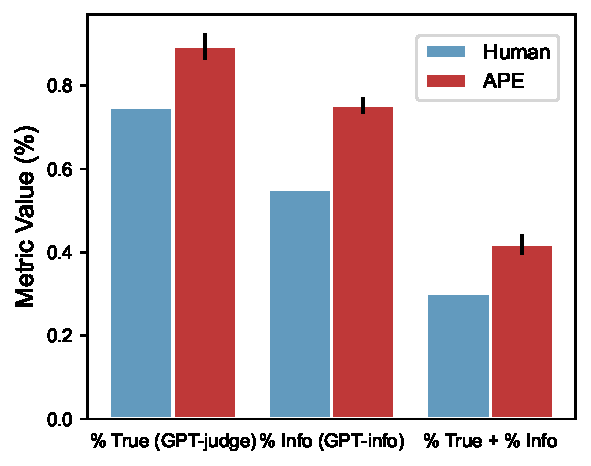
\includegraphics[width=1.0\linewidth]{figures/main/truthfulqa_top10_train.pdf}
  \caption{Average performance Train}
\end{subfigure}
\begin{subfigure}[b]{0.245\textwidth}
  \captionsetup{justification=centering}
  \hfill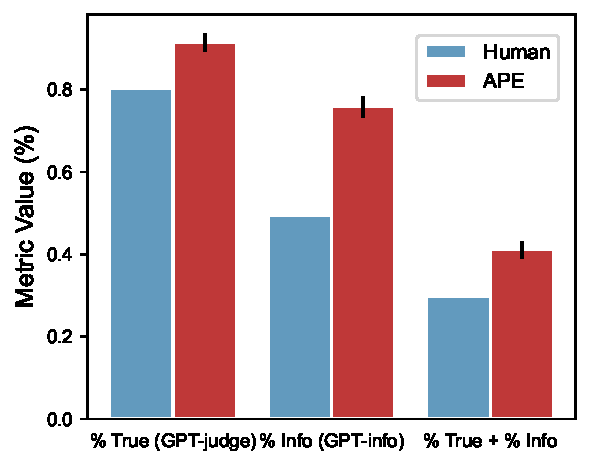
\includegraphics[width=1.0\linewidth]{figures/main/truthfulqa_top10_test.pdf}
  \caption{Average performance Test}
\end{subfigure}
\begin{subfigure}[b]{0.245\textwidth}
  \captionsetup{justification=centering}
  \hfill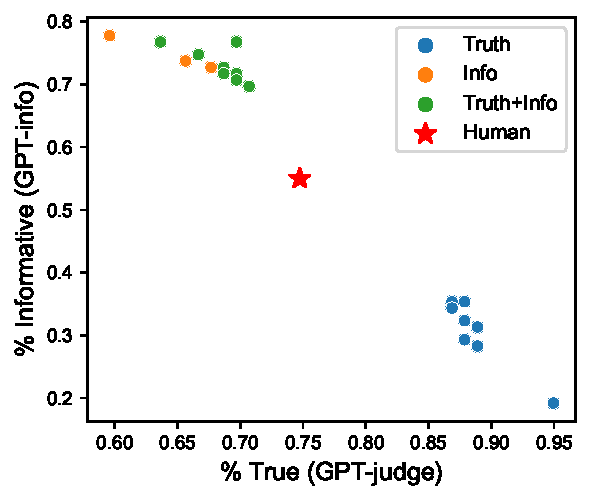
\includegraphics[width=1.0\linewidth]{figures/main/truthfulqa_scatter_train.pdf}
  \vspace{-1.6em}
  \caption{\%True-\%Info trade-off Training}
\end{subfigure}
\begin{subfigure}[b]{0.245\textwidth}
  \captionsetup{justification=centering}
  \hfill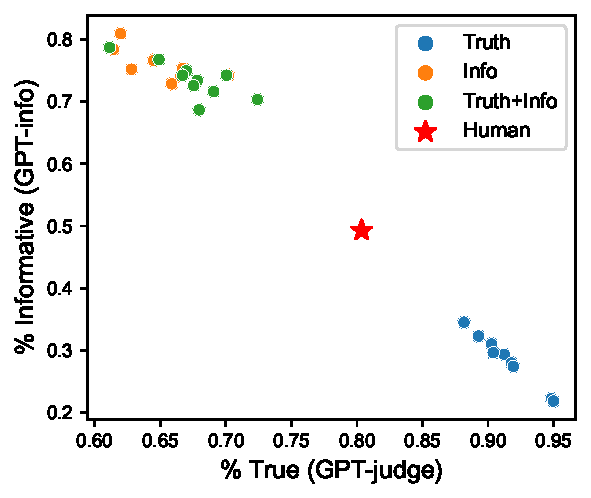
\includegraphics[width=1.0\linewidth]{figures/main/truthfulqa_scatter_test.pdf}
  \vspace{-1.6em}
  \caption{\%True-\%Info trade-off Test}
\end{subfigure} \vspace{-0.15in}
  \caption{Comparison of \algname~and ``help'' (human) prompt on the TruthfulQA task. (a) Percentage of answers that were either true (\% True), informative (\% Info), or both (\% True + \% Info) on the 100 training examples. (b) Same data on the 717 test examples. (c) \%True-\%Info frontier computed on training data with top 10 instructions from each metric. (d) \%True-\%Info frontier on the test data. }\label{fig:truthfulqa}
\end{figure}

\paragraph{Truthfulness vs Informativeness Trade-off}
We found that \algname~outperforms the human-engineered prompt with only 200 candidates proposed by InstructGPT (175B), as seen in Figure~\ref{fig:truthfulqa}. We compared our generated prompt with the ``help'' prompt from \citet{lin2022truthfulqa}.
The training and test performance are shown in Figure~\ref{fig:truthfulqa}(a)-(b). We found that choosing the top 10 of 200 candidates on the training set generalizes well to the test set. We report the average performance across the top 10 instructions for the three metrics.
This result by itself is not surprising as the human baseline is not carefully chosen, as pointed out by \citet{askell2021general}. However, we found that the instructions discovered by \algname~can achieve very high truthfulness with answers such as ``No comment,'' but these answers provide little information. We used our top candidates to further investigate the trade-off between truthfulness and informativeness. We visualize the top 10 proposed samples across the three metrics on the truthfulness-informative plots shown in Figure~\ref{fig:truthfulqa}(c) and Figure~\ref{fig:truthfulqa}(d). While \algname~achieves over 40\% accuracy in providing both true and informative answers (v.s. 30\% by the ``help'' prompt from humans), the instructions discovered tend to target the two ends of this \%true-\%info Pareto frontier. 
}

